% Created by tikzDevice version 0.12.6 on 2026-05-17 20:06:30
% !TEX encoding = UTF-8 Unicode
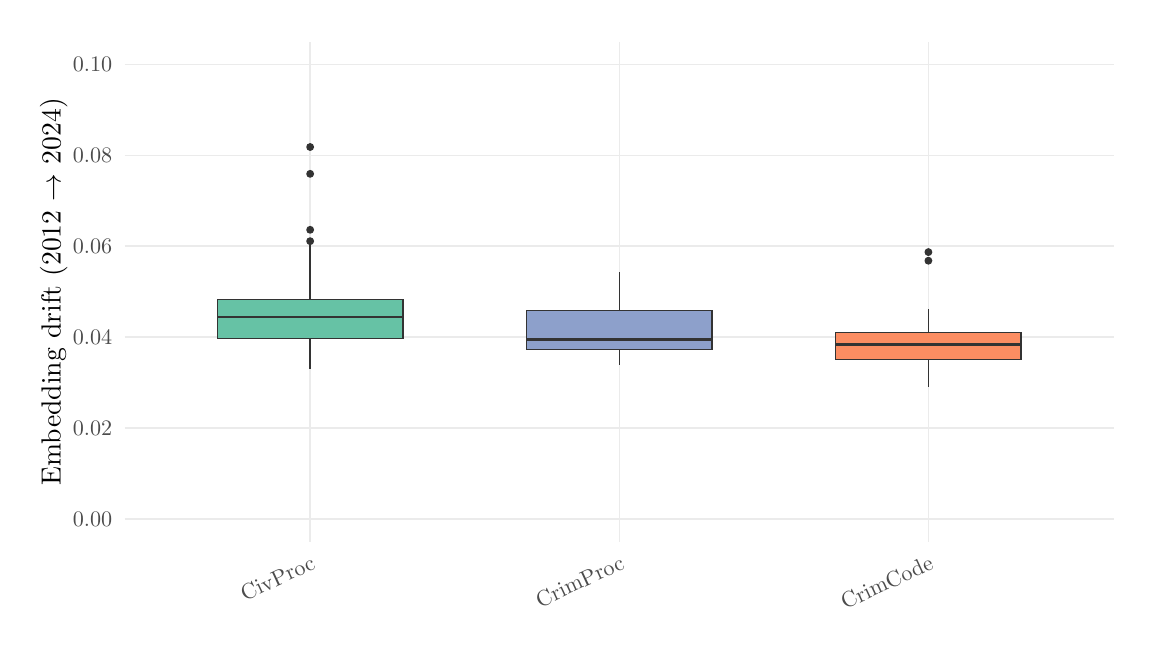
\begin{tikzpicture}[x=1pt,y=1pt]
\definecolor{fillColor}{RGB}{255,255,255}
\path[use as bounding box,fill=fillColor,fill opacity=0.00] (0,0) rectangle (397.48,216.81);
\begin{scope}
\path[clip] (  0.00,  0.00) rectangle (397.48,216.81);
\definecolor{fillColor}{RGB}{255,255,255}

\path[fill=fillColor] (  0.00,  0.00) rectangle (397.48,216.81);
\end{scope}
\begin{scope}
\path[clip] ( 35.05, 31.03) rectangle (392.48,211.81);
\definecolor{drawColor}{gray}{0.92}

\path[draw=drawColor,line width= 0.5pt,line join=round] ( 35.05, 39.25) --
	(392.48, 39.25);

\path[draw=drawColor,line width= 0.5pt,line join=round] ( 35.05, 72.12) --
	(392.48, 72.12);

\path[draw=drawColor,line width= 0.5pt,line join=round] ( 35.05,104.98) --
	(392.48,104.98);

\path[draw=drawColor,line width= 0.5pt,line join=round] ( 35.05,137.85) --
	(392.48,137.85);

\path[draw=drawColor,line width= 0.5pt,line join=round] ( 35.05,170.72) --
	(392.48,170.72);

\path[draw=drawColor,line width= 0.5pt,line join=round] ( 35.05,203.59) --
	(392.48,203.59);

\path[draw=drawColor,line width= 0.5pt,line join=round] (102.07, 31.03) --
	(102.07,211.81);

\path[draw=drawColor,line width= 0.5pt,line join=round] (213.77, 31.03) --
	(213.77,211.81);

\path[draw=drawColor,line width= 0.5pt,line join=round] (325.47, 31.03) --
	(325.47,211.81);
\definecolor{drawColor}{gray}{0.20}
\definecolor{fillColor}{gray}{0.20}

\path[draw=drawColor,line width= 0.4pt,line join=round,line cap=round,fill=fillColor] (102.07,173.68) circle (  1.21);

\path[draw=drawColor,line width= 0.4pt,line join=round,line cap=round,fill=fillColor] (102.07,139.66) circle (  1.21);

\path[draw=drawColor,line width= 0.4pt,line join=round,line cap=round,fill=fillColor] (102.07,143.77) circle (  1.21);

\path[draw=drawColor,line width= 0.4pt,line join=round,line cap=round,fill=fillColor] (102.07,163.99) circle (  1.21);

\path[draw=drawColor,line width= 0.5pt,line join=round] (102.07,118.50) -- (102.07,138.84);

\path[draw=drawColor,line width= 0.5pt,line join=round] (102.07,104.41) -- (102.07, 93.65);
\definecolor{fillColor}{RGB}{102,194,165}

\path[draw=drawColor,line width= 0.5pt,fill=fillColor] ( 68.56,118.50) --
	( 68.56,104.41) --
	(135.58,104.41) --
	(135.58,118.50) --
	( 68.56,118.50) --
	cycle;

\path[draw=drawColor,line width= 1.0pt] ( 68.56,112.30) -- (135.58,112.30);
\definecolor{fillColor}{gray}{0.20}

\path[draw=drawColor,line width= 0.4pt,line join=round,line cap=round,fill=fillColor] (325.47,132.60) circle (  1.21);

\path[draw=drawColor,line width= 0.4pt,line join=round,line cap=round,fill=fillColor] (325.47,135.72) circle (  1.21);

\path[draw=drawColor,line width= 0.5pt,line join=round] (325.47,106.63) -- (325.47,115.01);

\path[draw=drawColor,line width= 0.5pt,line join=round] (325.47, 96.93) -- (325.47, 86.91);
\definecolor{fillColor}{RGB}{252,141,98}

\path[draw=drawColor,line width= 0.5pt,fill=fillColor] (291.96,106.63) --
	(291.96, 96.93) --
	(358.98, 96.93) --
	(358.98,106.63) --
	(291.96,106.63) --
	cycle;

\path[draw=drawColor,line width= 1.0pt] (291.96,102.19) -- (358.98,102.19);

\path[draw=drawColor,line width= 0.5pt,line join=round] (213.77,114.52) -- (213.77,128.65);

\path[draw=drawColor,line width= 0.5pt,line join=round] (213.77,100.55) -- (213.77, 94.80);
\definecolor{fillColor}{RGB}{141,160,203}

\path[draw=drawColor,line width= 0.5pt,fill=fillColor] (180.26,114.52) --
	(180.26,100.55) --
	(247.28,100.55) --
	(247.28,114.52) --
	(180.26,114.52) --
	cycle;

\path[draw=drawColor,line width= 1.0pt] (180.26,104.16) -- (247.28,104.16);
\end{scope}
\begin{scope}
\path[clip] (  0.00,  0.00) rectangle (397.48,216.81);
\definecolor{drawColor}{gray}{0.30}

\node[text=drawColor,anchor=base east,inner sep=0pt, outer sep=0pt, scale=  0.80] at ( 30.55, 36.49) {0.00};

\node[text=drawColor,anchor=base east,inner sep=0pt, outer sep=0pt, scale=  0.80] at ( 30.55, 69.36) {0.02};

\node[text=drawColor,anchor=base east,inner sep=0pt, outer sep=0pt, scale=  0.80] at ( 30.55,102.23) {0.04};

\node[text=drawColor,anchor=base east,inner sep=0pt, outer sep=0pt, scale=  0.80] at ( 30.55,135.10) {0.06};

\node[text=drawColor,anchor=base east,inner sep=0pt, outer sep=0pt, scale=  0.80] at ( 30.55,167.97) {0.08};

\node[text=drawColor,anchor=base east,inner sep=0pt, outer sep=0pt, scale=  0.80] at ( 30.55,200.84) {0.10};
\end{scope}
\begin{scope}
\path[clip] (  0.00,  0.00) rectangle (397.48,216.81);
\definecolor{drawColor}{gray}{0.30}

\node[text=drawColor,rotate= 25.00,anchor=base east,inner sep=0pt, outer sep=0pt, scale=  0.80] at (104.40, 21.54) {CivProc};

\node[text=drawColor,rotate= 25.00,anchor=base east,inner sep=0pt, outer sep=0pt, scale=  0.80] at (216.10, 21.54) {CrimProc};

\node[text=drawColor,rotate= 25.00,anchor=base east,inner sep=0pt, outer sep=0pt, scale=  0.80] at (327.79, 21.54) {CrimCode};
\end{scope}
\begin{scope}
\path[clip] (  0.00,  0.00) rectangle (397.48,216.81);
\definecolor{drawColor}{RGB}{0,0,0}

\node[text=drawColor,rotate= 90.00,anchor=base,inner sep=0pt, outer sep=0pt, scale=  1.00] at ( 11.89,121.42) {Embedding drift (2012 $\to$ 2024)};
\end{scope}
\end{tikzpicture}
